\input{../../preamble2.tex}
\begin{document}
\begin{center}
	\Huge\textbf{Математический анализ}
\end{center}
\tableofcontents
\newpage
\begin{center}
\large{\textbf{Модуль №1} \\
\textit{Элементарные функции и пределы}}
\end{center}
\input{Основы математического анализа.tex}
\newpage
\zerocounter
\input{Числовая последовательность.tex}
\newpage
\zerocounter
\input{Предел функции.tex}
\newpage
\zerocounter
\input{бмф. Арифметические операции.tex}
\newpage
\zerocounter
\input{Предел функции. бмф ббф.tex}
\newpage
\zerocounter
\input{Непрерывность функции. Точки разрыва.tex}
\newpage
\zerocounter
\begin{center}
\large{\textbf{Модуль №2} \\
\textit{Дифференциальное исчисление функции одной переменной}}
\end{center}
\input{Производная функции.tex}
\newpage
\zerocounter
\input{Дифференциал функции.tex}
\zerocounter
\newpage
\input{Основные теоремы дифференциального исчисления.tex}
\newpage
\zerocounter
\input{Раскрытие неопределённостей.tex}
\zerocounter
\newpage
\input{Формула Тейлора.tex}
\zerocounter
\newpage
\input{Асимптоты.tex}
\zerocounter
%%%%%%%%%%%%%%%%%%%%
\section{Исследование функции $y = f(x)$ по первой производной}
\begin{definition}
	Функция $y=f(x)$, определённая на $(a;b)$, \textbf{возрастает} (\textbf{убывает}) на этом интервале, если: \[ \forall\ x_1, x_2 \in (a;b)\colon x_2 > x_1\ \Rightarrow\ f(x_2) > f(x_1)\quad \Big(f(x_2) < f(x_1)\Big) \]
\end{definition}
\begin{definition}
	Функция $y=f(x)$, определённая на $(a;b)$, \textbf{не убывает} (\textbf{не возрастает}) на этом интервале, если:
	\[ \forall\ x_1, x_2 \in (a;b)\colon x_2 > x_1\ \Rightarrow\ f(x_2) \ge f(x_1)\quad \Big(f(x_2) \le f(x_1)\Big) \]
\end{definition}
\begin{definition}
	Невозрастающая, неубывающая, возрастающая, убывающая функции называются \textbf{монотонными}.
\end{definition}
\begin{definition}
	Возрастающая и убывающая функции называются \textbf{строго монотонными}.
\end{definition}
\begin{theorem}[Необходимое и достаточное условие невозрастания | неубывания дифференцируеммой функции]
	Дифференцируемая на интервале $(a;b)$ функция $y=f(x)$ не возрастает (не убывает) на этом интервале тогда и только тогда, когда $\forall\ x \in (a;b)\colon$
	\[ f'(x) \le 0\quad \Big(f'(x) \ge 0\Big) \]
\end{theorem}
\begin{proof}[][Необходимость]
	\textbf{Дано}: $y=f(x)$ не \stackon{возрастает}{\footnotesize{(убывает)}} на $(a;b)$\\
	\textbf{Доказать}: $\forall x \in (a;b)\colon f'(x) \overset{\scriptsize{\big(\ge \big)}}{\le} 0$\\
	$\forall x \in (a;b)$\\
	$\Delta x$ --- приращение аргумента\\
	$x \to x + \Delta x$\\
	$\Delta y = y(x + \Delta x) - y(x)$ --- приращение функции\
	\newpage
	\noindent Случаи:
	\begin{enumerate}
		\item $\Delta x > 0$\\
		      Так как $y=f(x)$ не \stackon{возрастает}{\footnotesize{(убывает)}} на $(a;b)$: \vspace{-\topsep}
		      \begin{align*}
			                 & y(x+\Delta x) \overset{\scriptsize{\big(\ge \big)}}{\le} y(x)       \\
			      \Delta y = & y(x + \Delta x) - y(x) \overset{\scriptsize{\big(\ge \big)}}{\le} 0
		      \end{align*} \vspace{-\topsep}
		      Тогда:
		      \begin{gather*}
			      \boxed{\frac{\Delta y}{\Delta x} = \left(\frac{-}{+}\right) \overset{\scriptsize{\big(\ge \big)}}{\le} 0}
		      \end{gather*}
		\item $\Delta x < 0$\\
		      Так как $y=f(x)$ не \stackon{возрастает}{\footnotesize{(убывает)}} на $(a;b)$: \vspace{-\topsep}
		      \begin{align*}
			                 & y(x+\Delta x) \overset{\scriptsize{\big(\le \big)}}{\ge} y(x)       \\
			      \Delta y = & y(x + \Delta x) - y(x) \overset{\scriptsize{\big(\le \big)}}{\ge} 0
		      \end{align*} \vspace{-\topsep}
		      Тогда:
		      \begin{gather*}
			      \boxed{\frac{\Delta y}{\Delta x} = \left(\frac{+}{-}\right) \overset{\scriptsize{\big(\ge \big)}}{\le} 0}
		      \end{gather*}
	\end{enumerate}
	По теореме \textit{о предельном переходе в неравенстве} (\textbf{С.\pageref{Предельный переход в неравенстве}, Т.\ref{Предельный переход в неравенстве}}):
	\begin{gather*}
		\lim\limits_{\Delta x \to 0} \frac{\Delta y}{\Delta x} \overset{\scriptsize{\big(\ge \big)}}{\le} 0
	\end{gather*}
	По определению производной: $f'(x) \overset{\scriptsize{\big(\ge \big)}}{\le} 0$
\end{proof}
\begin{proof}[][Достаточность]
	\textbf{Дано}: $\forall x \in (a;b)\colon f'(x) \overset{\scriptsize{\big(\ge \big)}}{\le} 0$\\
	\textbf{Доказать}: $y=f(x)$ не \stackon{возрастает}{\footnotesize{(убывает)}} на $(a;b)$\\
	$\forall\ x_1, x_2 \in (a;b)\colon x_2 > x_1$\\
	Рассмотрим $[x_1; x_2]$.\\
	Функция $y=f(x)$ на $[x_1, x_2]$ удовлетворяет условиям теоремы \textit{Лагранжа} (\textbf{С.\pageref{Лагранж}, Т.\ref{Лагранж}}):
	\begin{enumerate}
		\item Непрерывность на $[x_1; x_2]$\\
		      По условию $y=f(x)$ дифференцируема на $(a;b)$. По теореме \textit{о связи дифференцируемости и непрерывности функции} (\textbf{С.\pageref{Связь диф. и непр. функции}}, Т.\ref{Связь диф. и непр. функции}) $\Rightarrow\ y=f(x)$ непрерывна на $[x_1; x_2]$.
		\item Дифференцируемость на $(x_1; x_2)$\\
		      Так как по условию. $y=f(x)$ дифференцируема на $(a;b)$, по теореме \textit{Лагранжа} $\exists\ c \in (x_1; x_2)$: \vspace{-\topsep}
		      \begin{gather*}
			      f'(c) = \frac{f(x_2) - f(x_1)}{x_2 - x_1}
		      \end{gather*}
		      Так как $x_2 > x_1$, то $x_2 - x_1 > 0$.\\
		      По условию $f'(x) \overset{\scriptsize{\big(\ge \big)}}{\le} 0$, $\forall x \in (a;b)\ \Rightarrow\ f'(c) \overset{\scriptsize{\big(\ge \big)}}{\le} 0$.\\
		      Тогда:
		      \begin{gather*}
			      f'(c) = \frac{f(x_2) - f(x_1)}{x_2 - x_1} \overset{\scriptsize{\big(\ge \big)}}{\le} 0\ \Rightarrow\ f(x_2) - f(x_1) \overset{\scriptsize{\big(\ge \big)}}{\le} 0 \text{ при } x_2 > x_1
		      \end{gather*}
	\end{enumerate} \vspace{-\topsep}
	$f(x_2) \overset{\scriptsize{\big(\ge \big)}}{\le} f(x_2)$ при $x_2 > x_1\ \Rightarrow$ по определению функция $y=f(x)$ не \stackon{возрастает}{\footnotesize{(убывает)}} на $(a;b)$.
\end{proof} \vspace{-11pt}
\begin{note}[\textbf{к доказательству}]
	Записи в скобках над словом или символом --- это то, что используется в доказательстве для неубывания.
\end{note}
\begin{theorem}[Необходимое условие строгой монотонности]
	Если дифференцируемая на $(a;b)$ функция $y=f(x)$ возрастает (убывает) на этом интервале, то $\forall x \in (a;b)\colon f'(x) \ge 0\quad \big( f'(x) \le 0 \big)$.
\end{theorem}
\begin{theorem}[Достаточное условие строгой монотонности]
	Если для дифференцируемой на $(a;b)$ функции $y=f(x)$ выполнены условия:
	\begin{enumerate}
		\item $\forall x \in (a;b)\colon f'(x) \ge 0\quad \big(f'(x) \le 0\big) $
		\item $f'(x)$ не обращается в нуль ни на каком промежутке $Y \le (a;b)$
	\end{enumerate}
	то функция $y=f(x)$ возрастает (убывает) на $(a;b)$.
\end{theorem}
\zerocounter
\section{Экстремумы функции}
\begin{definition}
	Пусть $y=f(x)$ определена на $(a;b),\ x_0 \in (a;b)$. Тогда:
	\begin{enumerate}
		\item Если $\exists\ \mathring{S}(x_0),\ \forall x \in \mathring{S}(x_0)\colon f(x) \le f(x_0)$, то \begin{tabular}{l} $x_0$ -- \textbf{точка локального максимума}, \\ $y_0 = y(x_0)$ -- \textbf{локальный максимум}. \end{tabular}
		\item Если $\exists\ \mathring{S}(x_0),\ \forall x \in \mathring{S}(x_0)\colon f(x) \ge f(x_0)$, то \begin{tabular}{l} $x_0$ -- \textbf{точка локального минимума}, \\ $y_0 = y(x_0)$ -- \textbf{локальный минимум}. \end{tabular}
	\end{enumerate}
\end{definition}
\begin{definition}
	Точки локального максимума и локального минимума называются \textbf{точками экстремума}.
\end{definition}
\begin{definition}
	Локальный максимум и локальный минимум называется \textbf{экстремумами}.
\end{definition}
\newpage
\begin{theorem}[Необходимое условие существования эксремума]
	Если функция $y=f(x)$ дифференцируема на $(a;b)$ и $x_0 \in (a;b)$ существует экстремум, то $f'(x_0) = 0$
\end{theorem}
\begin{eg}\ \\
	$y=x^2,\quad x_0 = 0$ --- точка минимума\\
	$y'=2x$\\
	$y'(0) = 0$ \vspace{-7\topsep}
	\begin{flushright}
		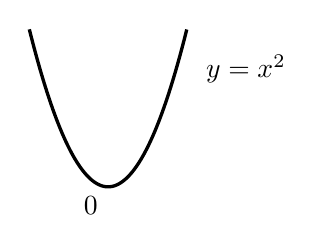
\begin{tikzpicture}[scale=0.5, thick]
			\tkzInit[xmin=-2.5, xmax=2.5, ymin=-1, ymax=4]
			\tkzDrawX \tkzDrawY
			\draw[domain=-2:2,smooth,variable=\x, samples=200, very thick] plot ({\x},{\x * \x});
			\node at (3.5, 3) {$y=x^2$};
			\node[below left] at (0, 0) {$0$};
		\end{tikzpicture}
	\end{flushright}
\end{eg}
\begin{eg}\ \\
	$y=x^3,\quad x_0 = 0$ --- не является точкой экстремума\\
	$y'=3x^2$\\
	$y'(0) = 0$ \vspace{-7\topsep}
	\begin{flushright}
		\begin{tikzpicture}[scale=0.5, thick]
			\tkzInit[xmin=-2, xmax=2, ymin=-3.5, ymax=3.5]
			\tkzDrawX \tkzDrawY
			\draw[domain=-1.5:1.5,smooth,variable=\x, samples=200, very thick] plot ({\x},{\x ^ 3});
			\node at (3.5, 3) {$y=x^3$};
			\node[below left] at (0, 0) {\footnotesize $0$};
		\end{tikzpicture}
	\end{flushright}
\end{eg}
\begin{definition}
	Точки, в которых производная функции обращается в нуль, называются \textbf{стационарными}.
	\begin{gather*}
		f'(x_0) = 0\qquad x_0 \text{ --- стационарная точка}
	\end{gather*}
\end{definition}
\begin{definition}
	Точки, в которых производная функции обращается в нуль или не существует, называются \textbf{критическими точками 1-го порядка}.
\end{definition}
\begin{eg}\ \\
	$y=|x|,\quad x_0 = 0$ --- точка минимума.\\
	$\nexists\ y'$\\
	$y'_+ = 1$\\
	$y'_- = -1$ \vspace{-8\topsep}
	\begin{flushright}
		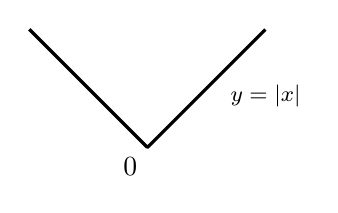
\begin{tikzpicture}[scale = 0.5, thick]
			\tkzInit[xmin=-3.5, xmax=3.5, ymin=-1, ymax=3.5]
			\tkzDrawX \tkzDrawY
			\draw[domain=-3:3,smooth,variable=\x, samples=200, very thick] plot ({\x},{abs(\x)});
			\node at (3, 1.3) {\footnotesize $y = |x|$};
			\node[below left] at (0, 0) {$0$};
		\end{tikzpicture}
	\end{flushright}
\end{eg}
\begin{eg}\ \\
	$y = x^{\tfrac{2}{3}},\quad x_0 = 0$ --- точка минимума.\\[1ex]
	$\displaystyle y' = \frac{2}{3}\cdot x^{-\tfrac{1}{3}} = \frac{2}{3\sqrt[3]{x}}$\\
	$y'(0) = \nexists $
	\begin{flushright}\vspace{-8\topsep}
		\begin{tikzpicture}[scale = 0.5, thick]
			\tkzInit[xmin=-3.5, xmax=3.5, ymin=-1, ymax=3.5]
			\tkzDrawX \tkzDrawY
			\draw[domain=-3:3,smooth,variable=\x, samples=200, very thick] plot ({\x},{pow(abs(\x), 2/3)});
			\node at (3, 1) {\footnotesize $y = x^{\tfrac{2}{3}}$};
			\node[below left] at (0, 0) {$0$};
		\end{tikzpicture}
	\end{flushright}
\end{eg}
\subsection*{Вывод}
Точки экстремума могут быть двух видов:
\begin{enumerate}
	\item $f'(x) = 0$ --- \textbf{гладкий экстремум};
	\item $\nexists f'(x)$ --- \textbf{острый экстремум}.
\end{enumerate}
\begin{theorem}[Первый достаточный признак локального экстремума]
	Пусть $y=f(x)$ непрерывна в $S(x_0)$, где $x_0$ --- критическая точка 1-го порядка; дифференцируема в $\mathring{S}(x_0)$. Тогда если производная функции меняет свой знак при переходе через точку $x_0$, то $x_0$ --- точка экстремума. Причём:
	\begin{enumerate}
		\item если при $x < x_0\colon f'(x) > 0$, а при $x > x_0\colon f'(x) < 0$, то $x_0$ --- точка максимума;
		\item если при $x < x_0\colon f'(x) < 0$, а при $x > x_0\colon f'(x) > 0$, то $x_0$ --- точка минимума.
	\end{enumerate}
\end{theorem}
\begin{proof}
	$\forall x \in S(x_0)$.\\
	$\bullet$ Пусть $x > x_0$. Рассмотрим $[x_0; x]$. \\
	Тогда функция $y=f(x)$ удовлетворяет условиям теоремы \textit{Лагранжа} (\textbf{С.\pageref{Лагранж}, Т.\ref{Лагранж}}):
	\begin{enumerate}
		\item непрерывна на $[x_0; x]$\\
		      По условию функция непрерывна в $S(x_0)\ \Rightarrow\ y=f(x)$ непрерывна на $[x_0; x]$.
		\item дифференцируема на $(x_0; x)$\\
		      По условию $y=f(x)$ дифференцируема в $\mathring{S}(x_0)\ \Rightarrow\ y=f(x)$ дифференцируема на $(x_0; x)$.
	\end{enumerate}
	По теореме \textit{Лагранжа} $\displaystyle \exists\ c \in (x_0; x)\colon f(c) = \frac{f(x) - f(x_0)}{x - x_0}$\\
	Так как $x > x_0$, то $x - x_0 > 0$.\\
	По условию 1) при $x > x_0\colon f'(x) \overset{\scriptsize{\big(>\big)}}{<} 0\ \Rightarrow$
	\begin{gather*}
		\Rightarrow\ f'(c) = \frac{f(x) - f(x_0)}{x - x_0} \overset{\scriptsize{\big(>\big)}}{<} 0\ \Rightarrow\ f(x) - f(x_0) \overset{\scriptsize{\big(>\big)}}{<} 0\ \Rightarrow\ f(x) \overset{\scriptsize{\big(>\big)}}{<} f(x_0)
	\end{gather*}
	По определению строгого \stackon{максимума}{\footnotesize{(минимума)}}, $x_0$ --- точка \stackon{максимума}{\footnotesize{(минимума)}}.\\
	$\bullet$ Пусть $x<x_0$, тогда рассматриваем $[x; x_0]$.\\
	$y=f(x)$ на $[x; x_0]$ удовлетворяет теореме \textit{Лагранжа}.\\[1ex]
	По теореме \textit{Лагранжа}: $\displaystyle \exists\ c \in (x; x_0)\colon f'(c) = \frac{f(x_0) - f(x)}{x_0 - x}$\\[1ex]
	Так как $x < x_0$, то $x - x_0 < 0\ \Rightarrow\ x_0-x > 0$.\\
	По условию 1) при $x < x_0\colon f'(x) \overset{\scriptsize{\big(<\big)}}{>} 0\ \Rightarrow$
	\begin{gather*}
		\Rightarrow\ f'(c) = \frac{f(x_0) - f(x)}{x_0 - x} \overset{\scriptsize{\big(<\big)}}{>} 0\ \Rightarrow\ f(x_0) - f(x) \overset{\scriptsize{\big(<\big)}}{>} 0\ \Rightarrow\ f(x_0) \overset{\scriptsize{\big(<\big)}}{>} f(x)
	\end{gather*}
	По определению строго локального максимума, $x_0$ --- точка строгого локального\\[1ex]
	\stackon{максимума}{\footnotesize{(минимума)}} $\Rightarrow\ \forall x \in S(x_0)\colon x_0$ --- точка строгого локального \stackon{максимума}{\footnotesize{(минимума)}}.
\end{proof} \vspace{-11pt}
\begin{note}[{\textbf{к доказательству}}]
	Записи в скобках над словом или символом --- это то, что используется в доказательстве для случая строго локального минимума.
\end{note}
\newpage
\begin{theorem}[Второй достаточный признак локального экстремума]
	Пусть функция $y=f(x)$ дважды дифференцируема в точке $x_0$ и $f'(x_0) = 0$. Тогда:
	\begin{enumerate}
		\item если $f''(x_0) < 0$, то $x_0$ --- точка строгого максимума;
		\item если $f''(x_0) > 0$, то $x_0$ --- точка строгого минимума.
	\end{enumerate}
\end{theorem}
\begin{proof}
	Представим функцию $y=f(x)$ в $S(x_0)$ по формуле Тейлора:
	\begin{align*}
		f(x) = f(x_0) + \frac{f'(x_0)}{1!}\cdot (x-x_0) +  \frac{f''(x_0)}{2!}\cdot (x-x_0)^2 + o\left((x-x_0)^2\right)
	\end{align*}
	Так как $f'(x_0) = 0$, то:
	\begin{align*}
		f(x)          & = f(x_0) + \frac{f''(x_0)}{2!}\cdot (x-x_0)^2 + o\left((x-x_0)^2\right) \\
		f(x) - f(x_0) & = \frac{f''(x_0)}{2!}\cdot (x-x_0)^2 + o\left((x-x_0)^2\right)
	\end{align*}
	Знак $f(x) - f(x_0)$ определяет $f''(x_0)$, так как $o\left((x-x_0)^2\right)$ --- б.м.ф. при $x\to x_0$.\\
	Тогда:
	\begin{enumerate}
		\item если $f''(x_0) < 0$, то $f(x) - f(x_0) < 0\ \Rightarrow\ f(x) < f(x_0),\ \forall x \in S(x_0)$, по определению строгого локального максимума $x_0$ --- точка строго локального максимума;
		\item если $f''(x_0) > 0$, то $f(x) - f(x_0) > 0\ \Rightarrow\ f(x) > f(x_0)\quad \forall x \in S(x_0)$, по определению строгого локального минимума $x_0$ --- точка строгого локального минимума.
	\end{enumerate}
\end{proof}
\zerocounter
\section{Исследование функции $y=f(x)$ по второй производной}
\begin{definition}
	Говорят, что график функции $y=f(x)$ на интервале $(a;b)$ \textbf{выпуклый} или \textbf{выпуклый вверх} на этом интервале, если касательная к нему в любой точке этого интервала лежит выше графика функции.
\end{definition}
\begin{definition}
	Говорят, что график функции $y=f(x)$ на интервале $(a;b)$ \textbf{вогнутый} или \textbf{выпуклый вниз} на этом интервале, если касательная к нему в любой точке этого интервала лежит ниже графика функции.
\end{definition}
%%%%%%%%%%%%%%%%%%%%
\end{document}